\chapter{Appendix}
\label{chap:appendix}
In this appendix are collected all results of
\begin{itemize}
    \item feature selection evaluated by fs\_results.ipynb;
    \item model prediction errors computed with:
    \begin{itemize}
        \item Keras\_prediction\_model.ipynb;
        \item RandomForest\_prediction\_model.ipynb;
    \end{itemize}  
\end{itemize}
\section{Feature Selection results}
\subsection{Borda Count results}
\begin{figure}[H]
\centering
\subfloat[10 Km resolution with mountains]{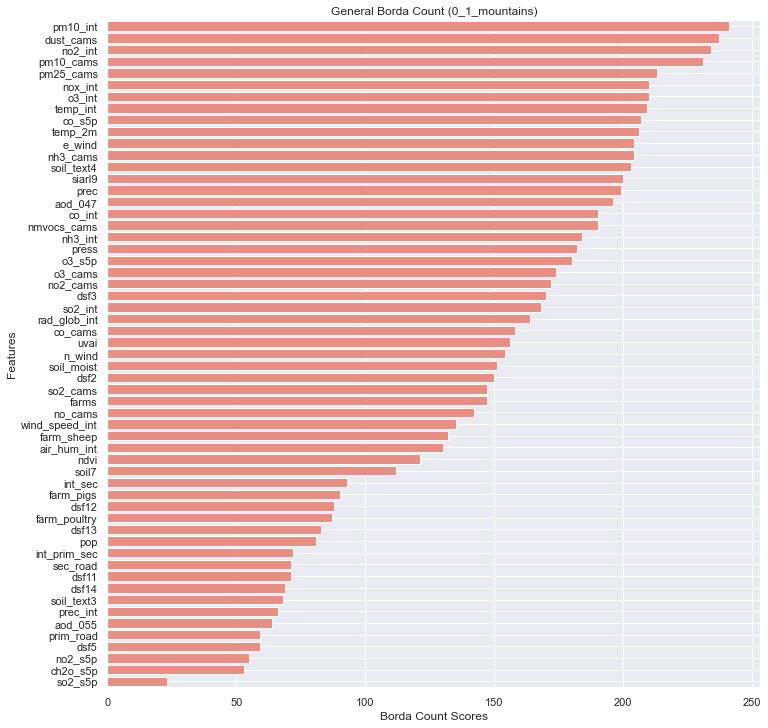
\includegraphics[scale =0.40]{images/tests/0_1_mountainspm25_st.png}}\\
\subfloat[10 Km resolution with mountains]{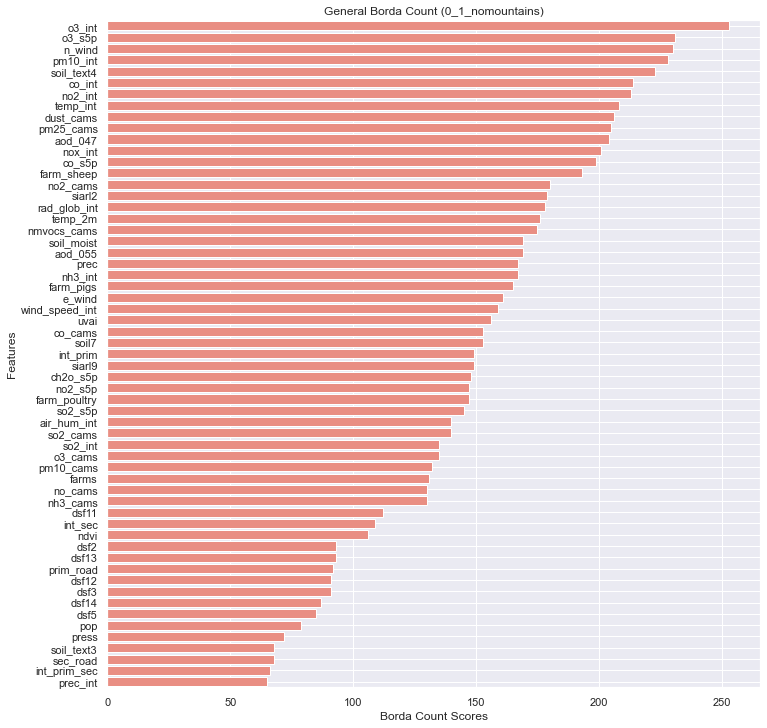
\includegraphics[scale =0.40]{images/tests/0_1_nomountainspm25_st.png}}
\caption{FS results obtained with fine particulate ('pm25\_st') as target variable and 10 km resolution. The results are averaged over the 5 periods. }
\end{figure}
\begin{figure}[H]
\centering
\subfloat[1 Km resolution with mountains]{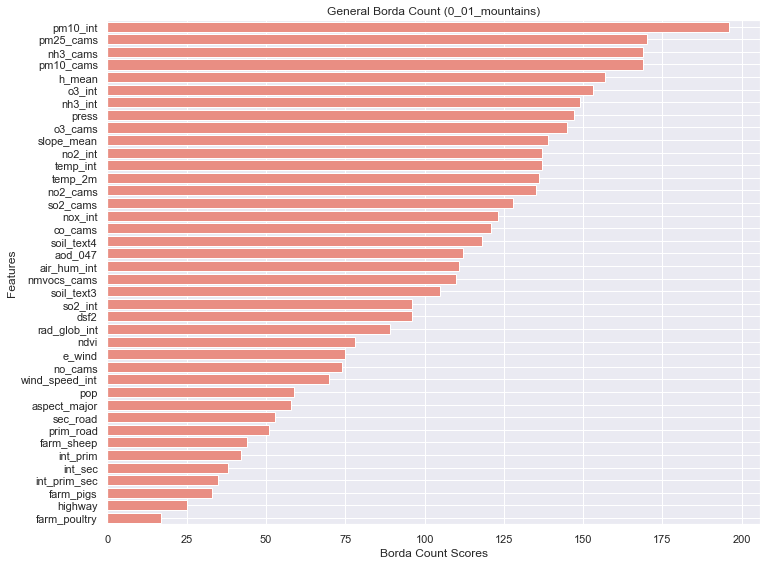
\includegraphics[scale =0.42]{images/tests/0_01_mountainspm25_st.png}}\\
\subfloat[1 Km resolution with mountains]{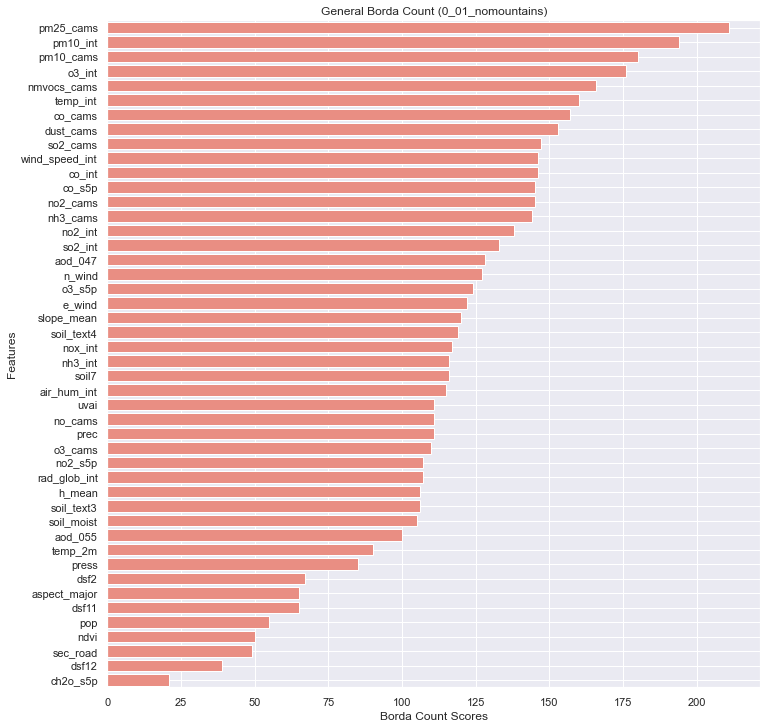
\includegraphics[scale =0.42]{images/tests/0_01_nomountainspm25_st.png}}
\caption{FS results obtained with fine particulate ('pm25\_st') as target variable and 1 km resolution. The results are averaged over the 5 periods.}
\end{figure}
\begin{figure}[H]
\centering
\subfloat[10 Km resolution with mountains]{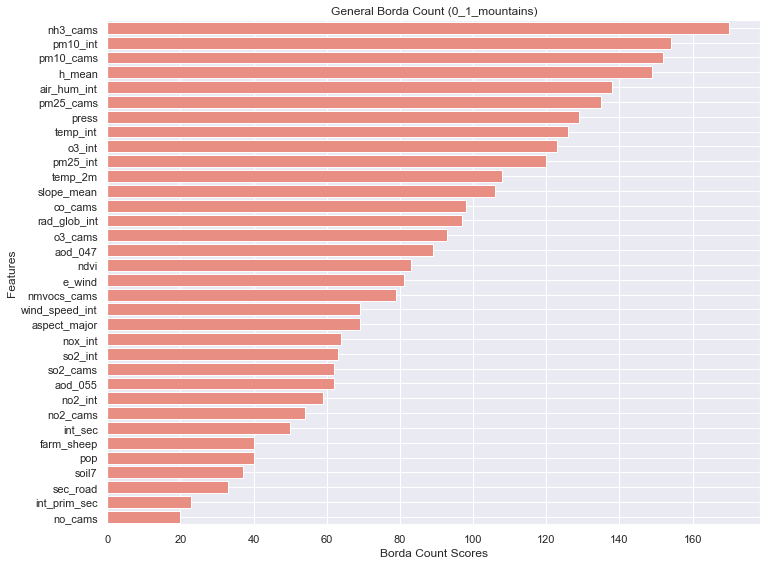
\includegraphics[scale =0.42]{images/tests/0_1_mountainsnh3_st.png}}\\
\subfloat[10 Km resolution with mountains]{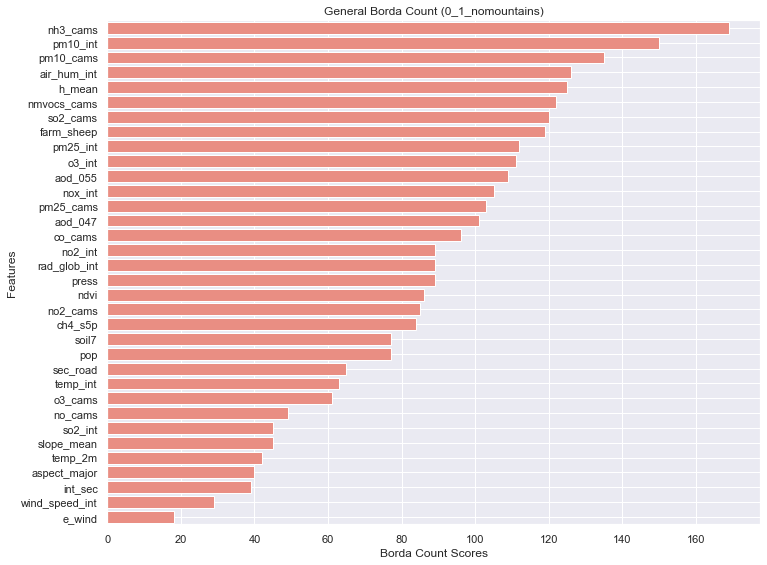
\includegraphics[scale =0.42]{images/tests/0_1_nomountainsnh3_st.png}}
\caption{FS results obtained with ammonia ('nh3\_st') as target variable and 10 km resolution. The results are averaged over the 5 periods.}
\end{figure}
\begin{figure}[H]
\centering
\subfloat[1 Km resolution with mountains]{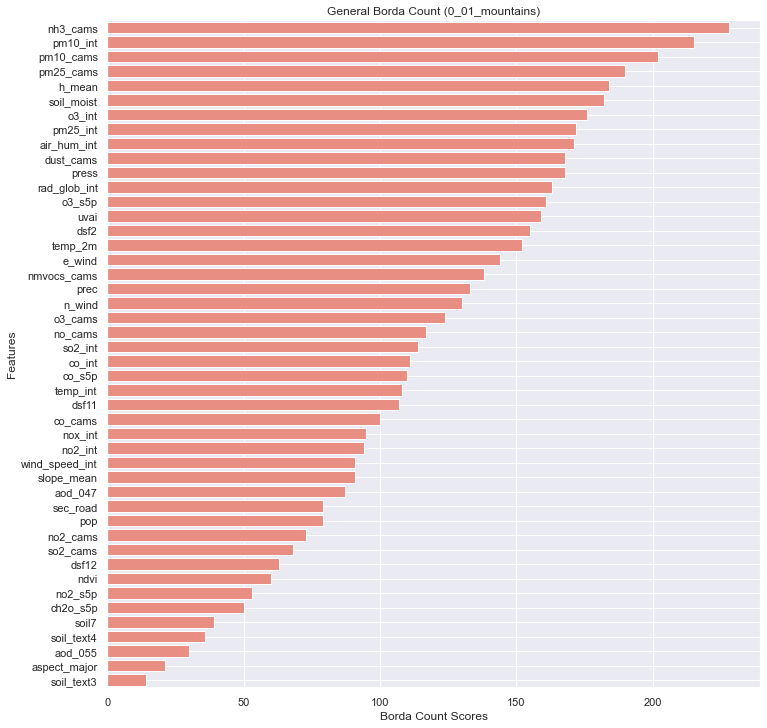
\includegraphics[scale =0.42]{images/tests/0_01_mountainsnh3_st.png}}\\
\subfloat[1 Km resolution with mountains]{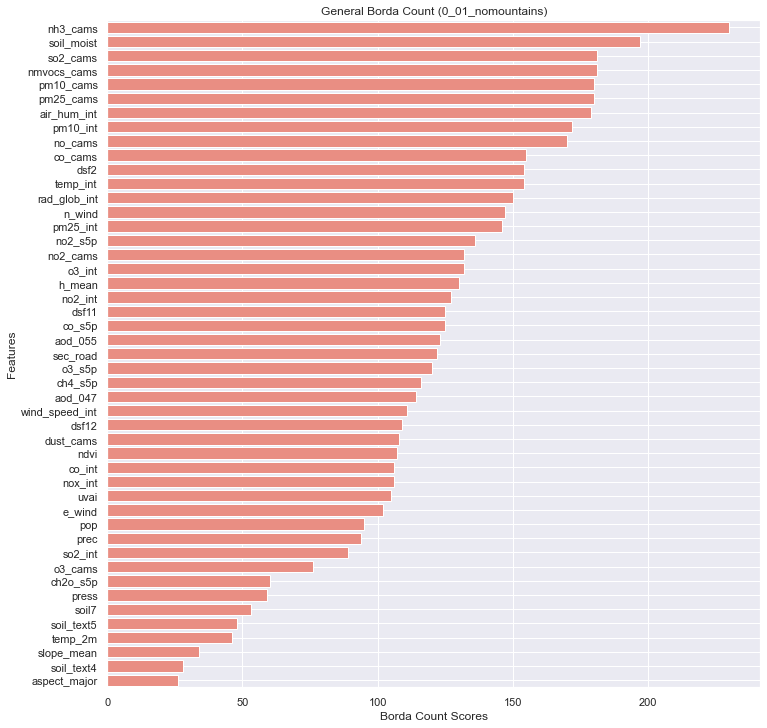
\includegraphics[scale =0.42]{images/tests/0_01_nomountainsnh3_st.png}}
\caption{FS results obtained with ammonia ('nh3\_st') as target variable and 1 km resolution. The results are averaged over the 5 periods.}
\end{figure}
\subsection{Pearson correlation index results}
\begin{figure}[H]
    \centering
    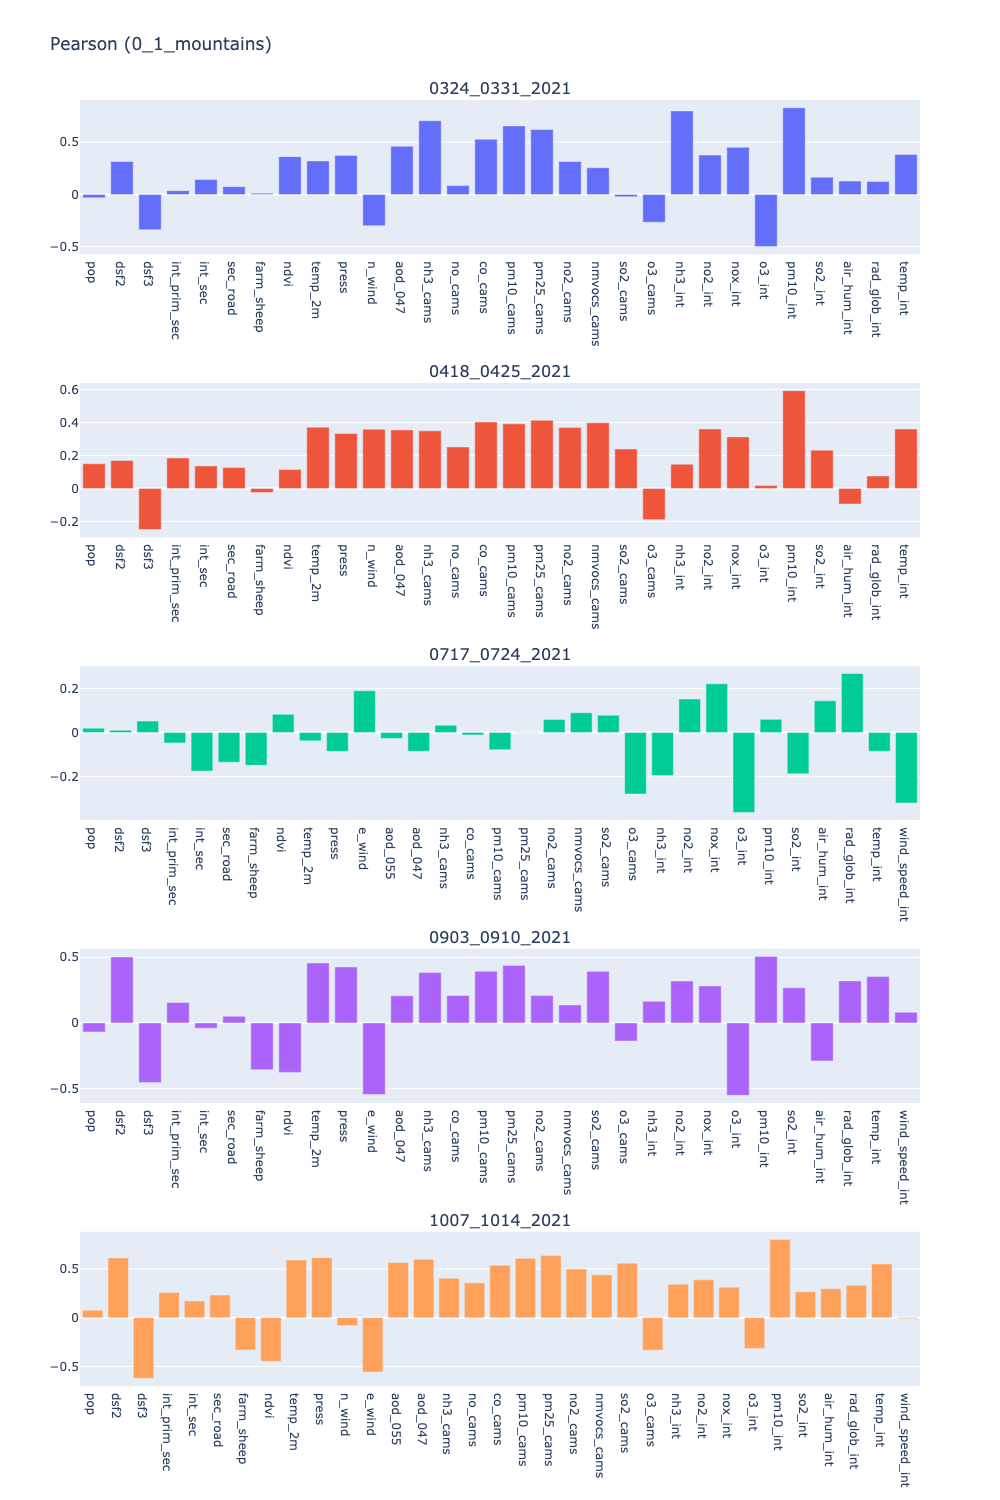
\includegraphics[scale=0.38]{images/tests/0_1_mountainspm25_st_pearson.png}
    \caption{Pearson correlation index results with respect to fine particulate ('pm25\_st') as target variable, with 10km resolution including mountains in each period. }
\end{figure}
\begin{figure}[H]
    \centering
    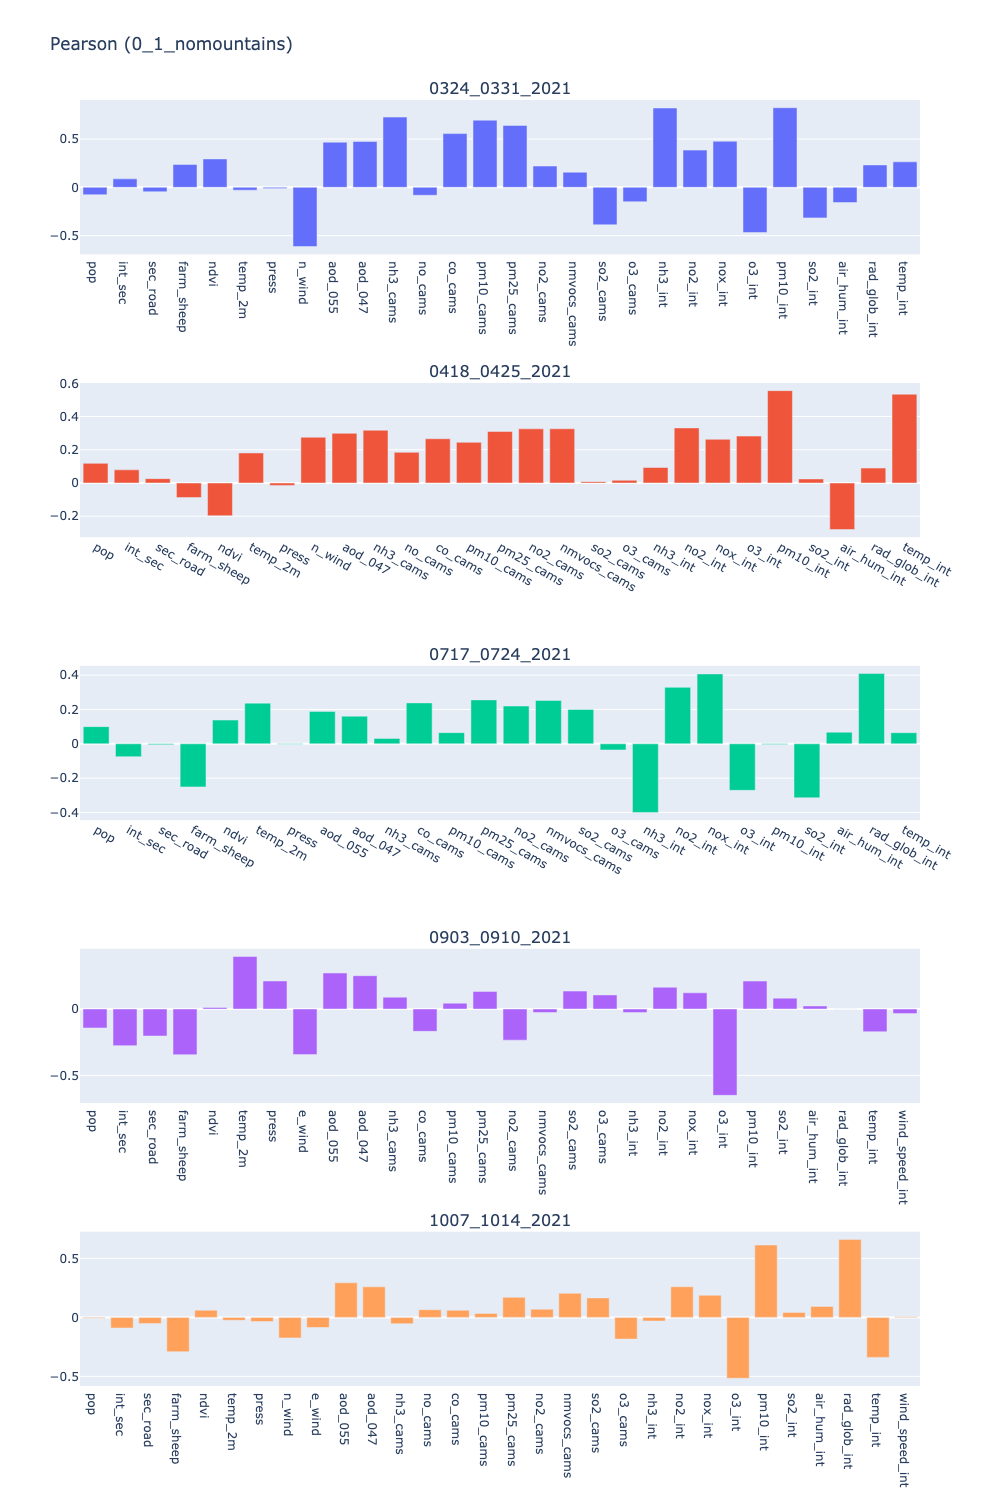
\includegraphics[scale=0.38]{images/tests/0_1_nomountainspm25_st_pearson.png}
    \caption{Pearson correlation index results with respect to fine particulate ('pm25\_st') as target variable, with 10km resolution excluding mountains in each period.}
    
\end{figure}
\begin{figure}[H]
    \centering
    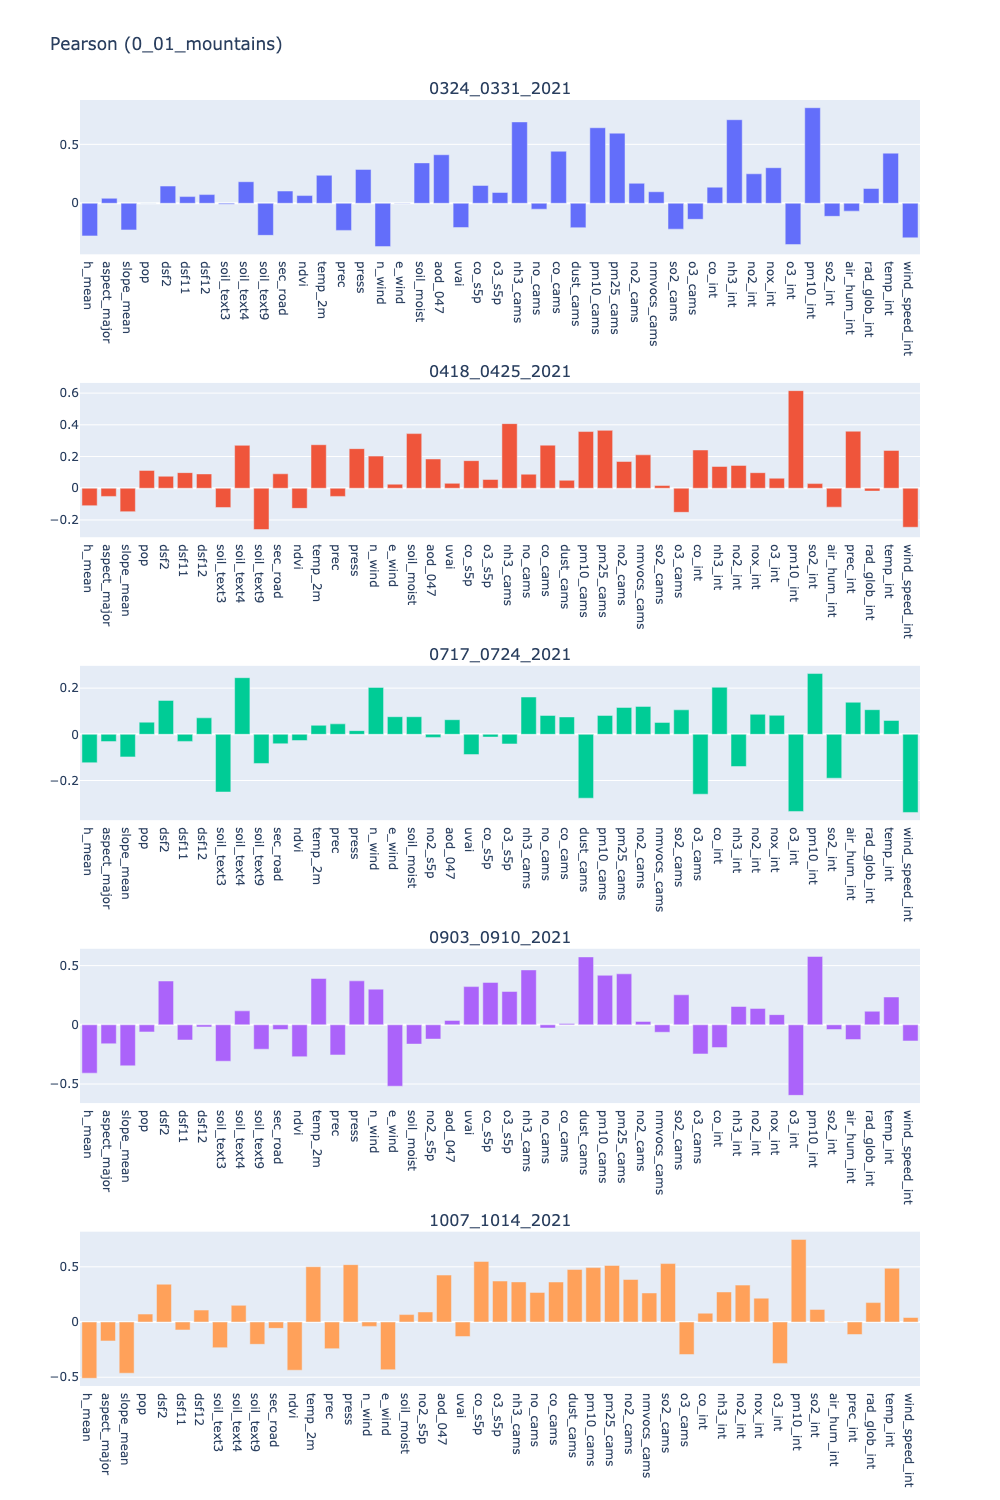
\includegraphics[scale=0.38]{images/tests/0_01_mountainspm25_st_pearson.png}
    \caption{Pearson correlation index results with respect to fine particulate ('pm25\_st') as target variable, with 1km resolution including mountains in each period.}
    
\end{figure}
\begin{figure}[H]
    \centering
    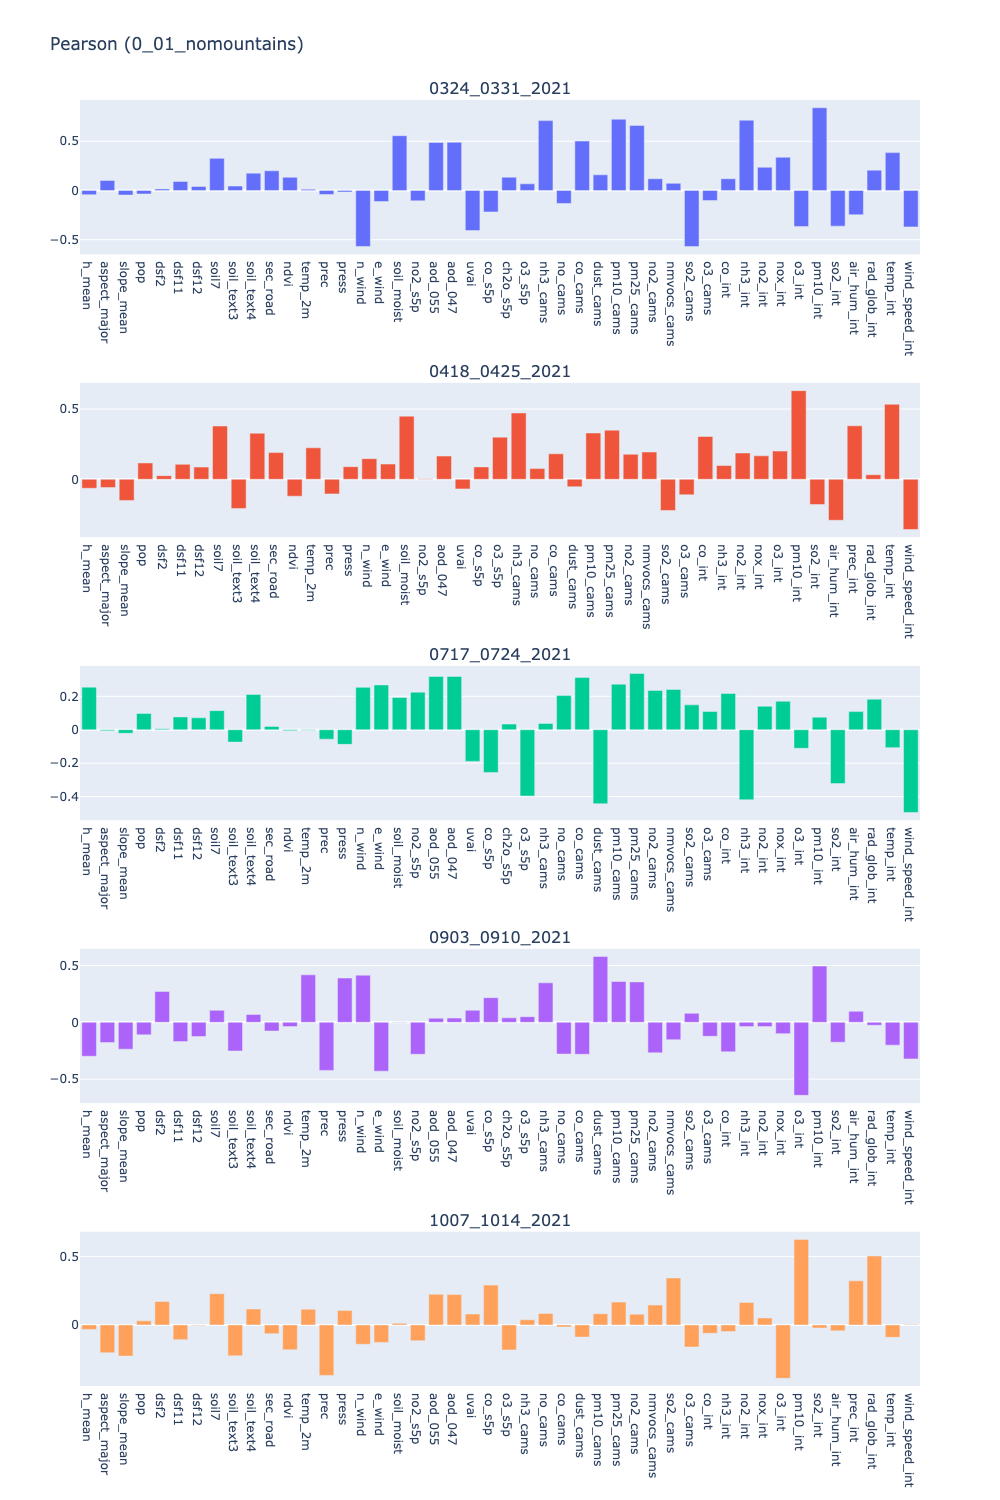
\includegraphics[scale=0.38]{images/tests/0_01_nomountainspm25_st_pearson.png}
    \caption{Pearson correlation index results with respect to fine particulate ('pm25\_st') as target variable, with 1km resolution excluding mountains in each period.}
    
\end{figure}


\begin{figure}[H]
    \centering
    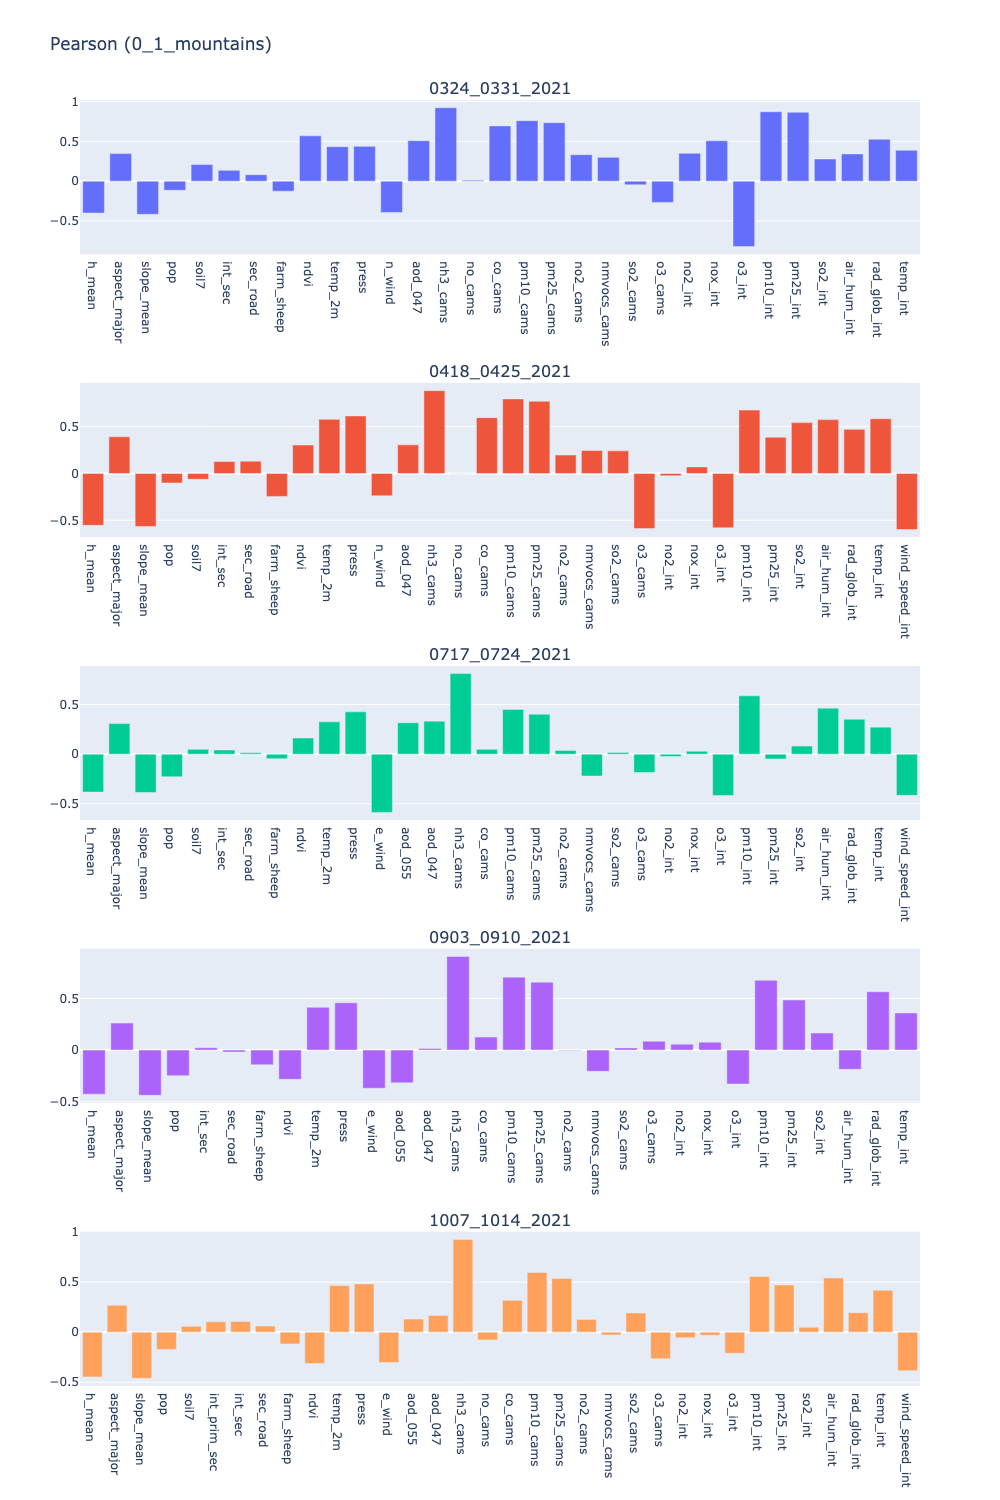
\includegraphics[scale=0.38]{images/tests/0_1_mountainsnh3_st_pearson.png}
    \caption{Pearson correlation index results with respect to ammonia ('nh3\_st') as target variable, with 10km resolution including mountains in each period.}
    
\end{figure}
\begin{figure}[H]
    \centering
    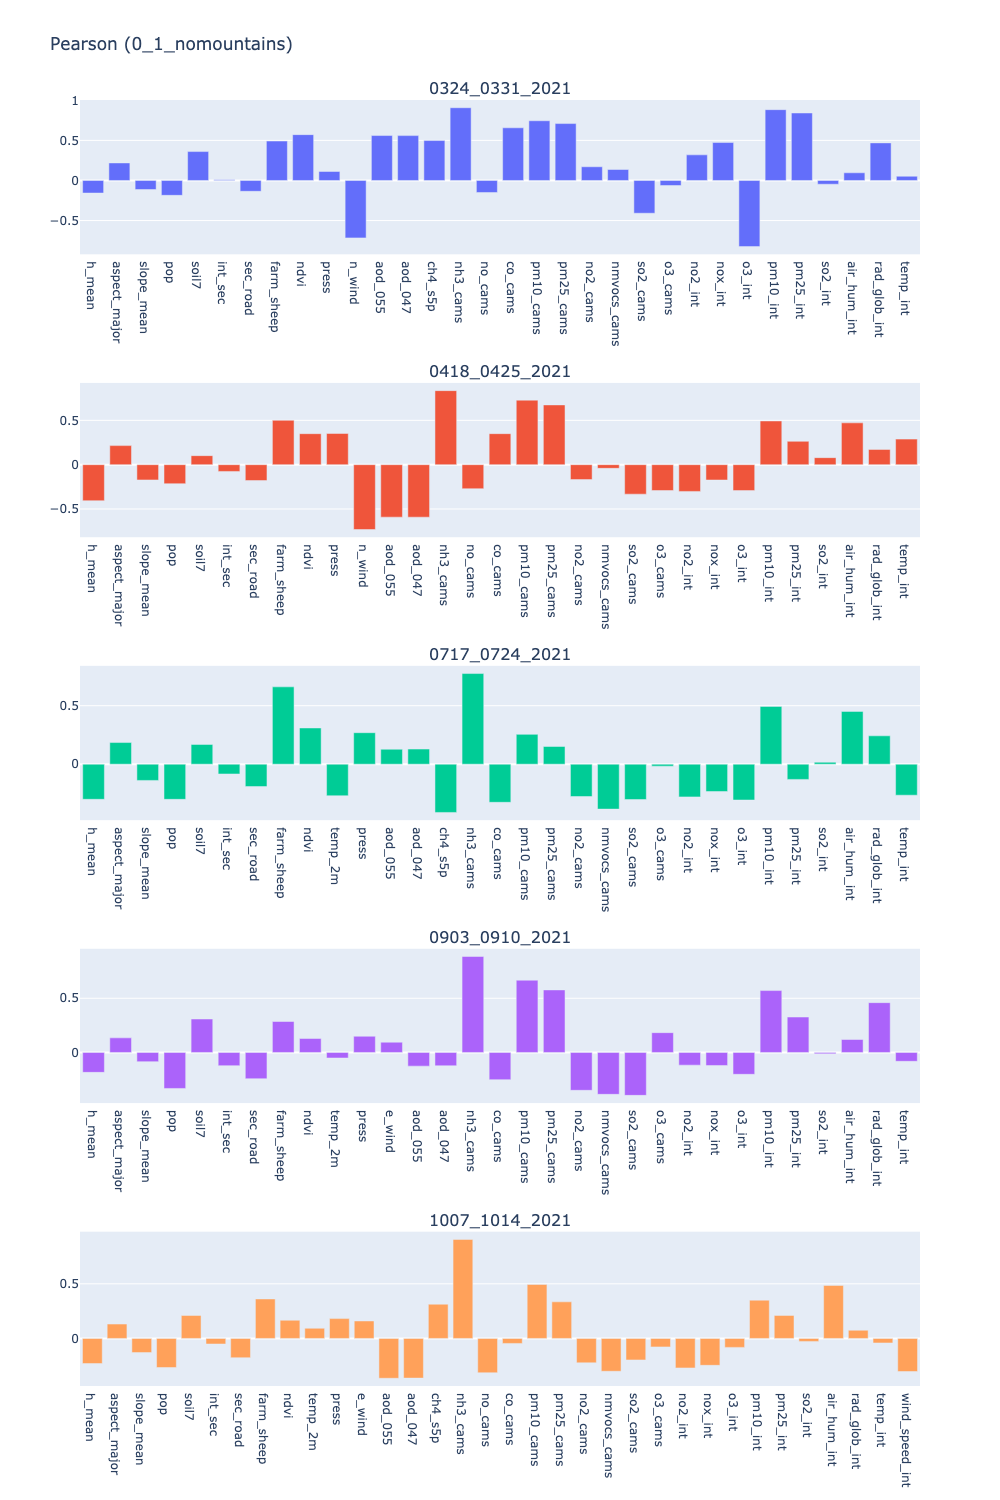
\includegraphics[scale=0.38]{images/tests/0_1_nomountainsnh3_st_pearson.png}
    \caption{Pearson correlation index results with respect to ammonia ('nh3\_st') as target variable, with 10km resolution excluding mountains in each period.}
    
\end{figure}
\begin{figure}[H]
    \centering
    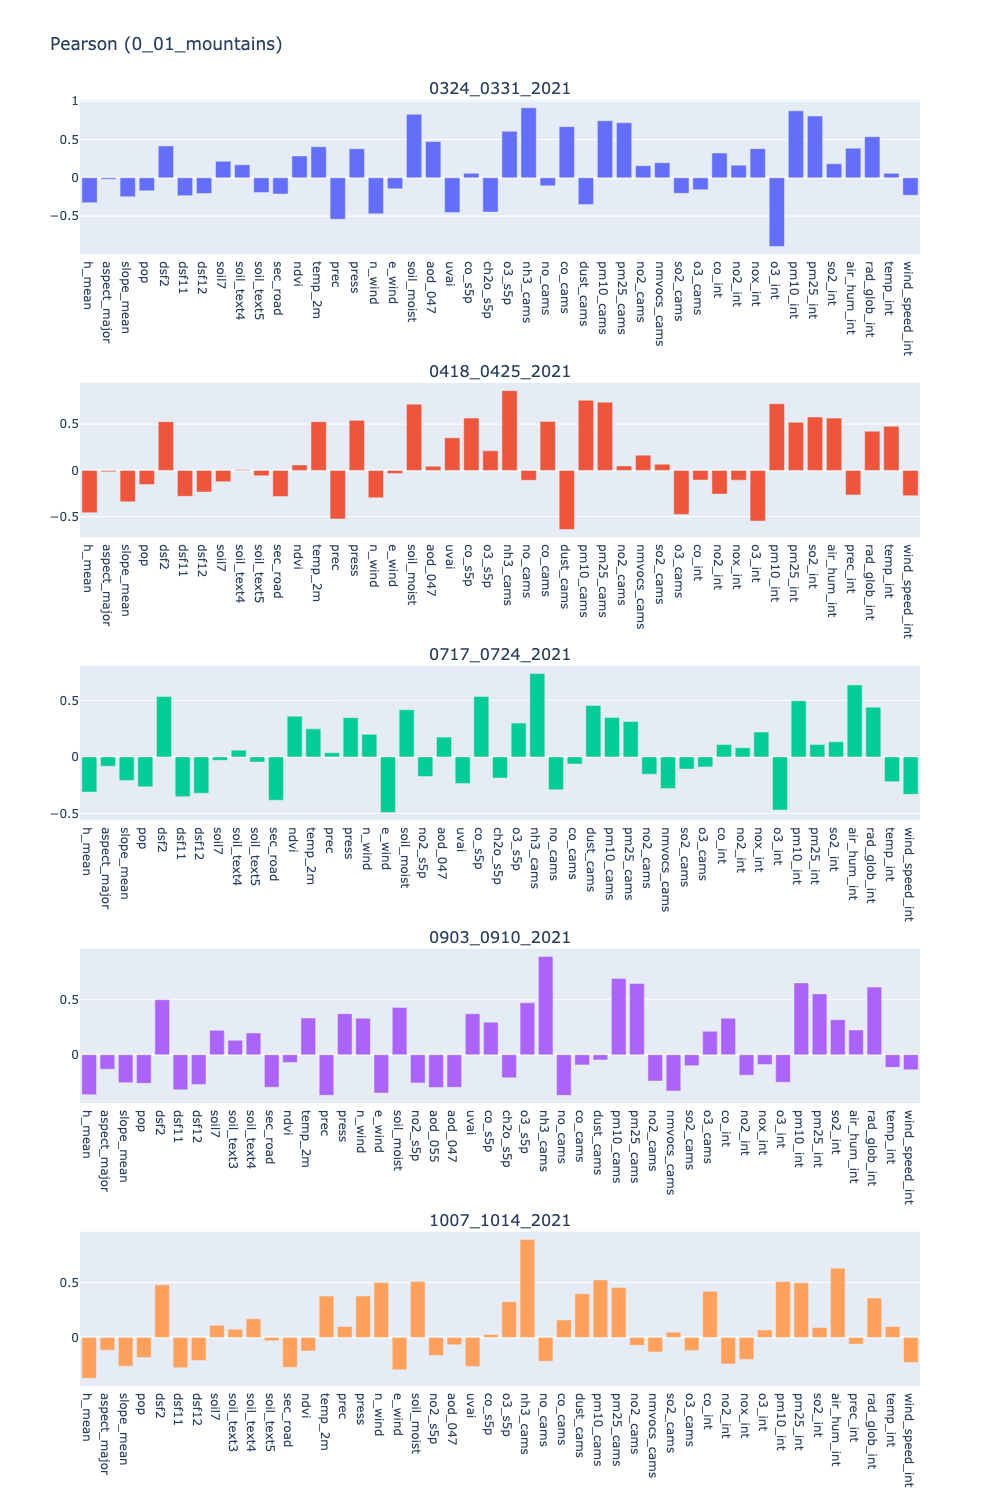
\includegraphics[scale=0.38]{images/tests/0_01_mountainsnh3_st_pearson.png}
    \caption{Pearson correlation index results with respect to ammonia ('nh3\_st') as target variable, with 1km resolution including mountains in each period.}
    
\end{figure}
\begin{figure}[H]
    \centering
    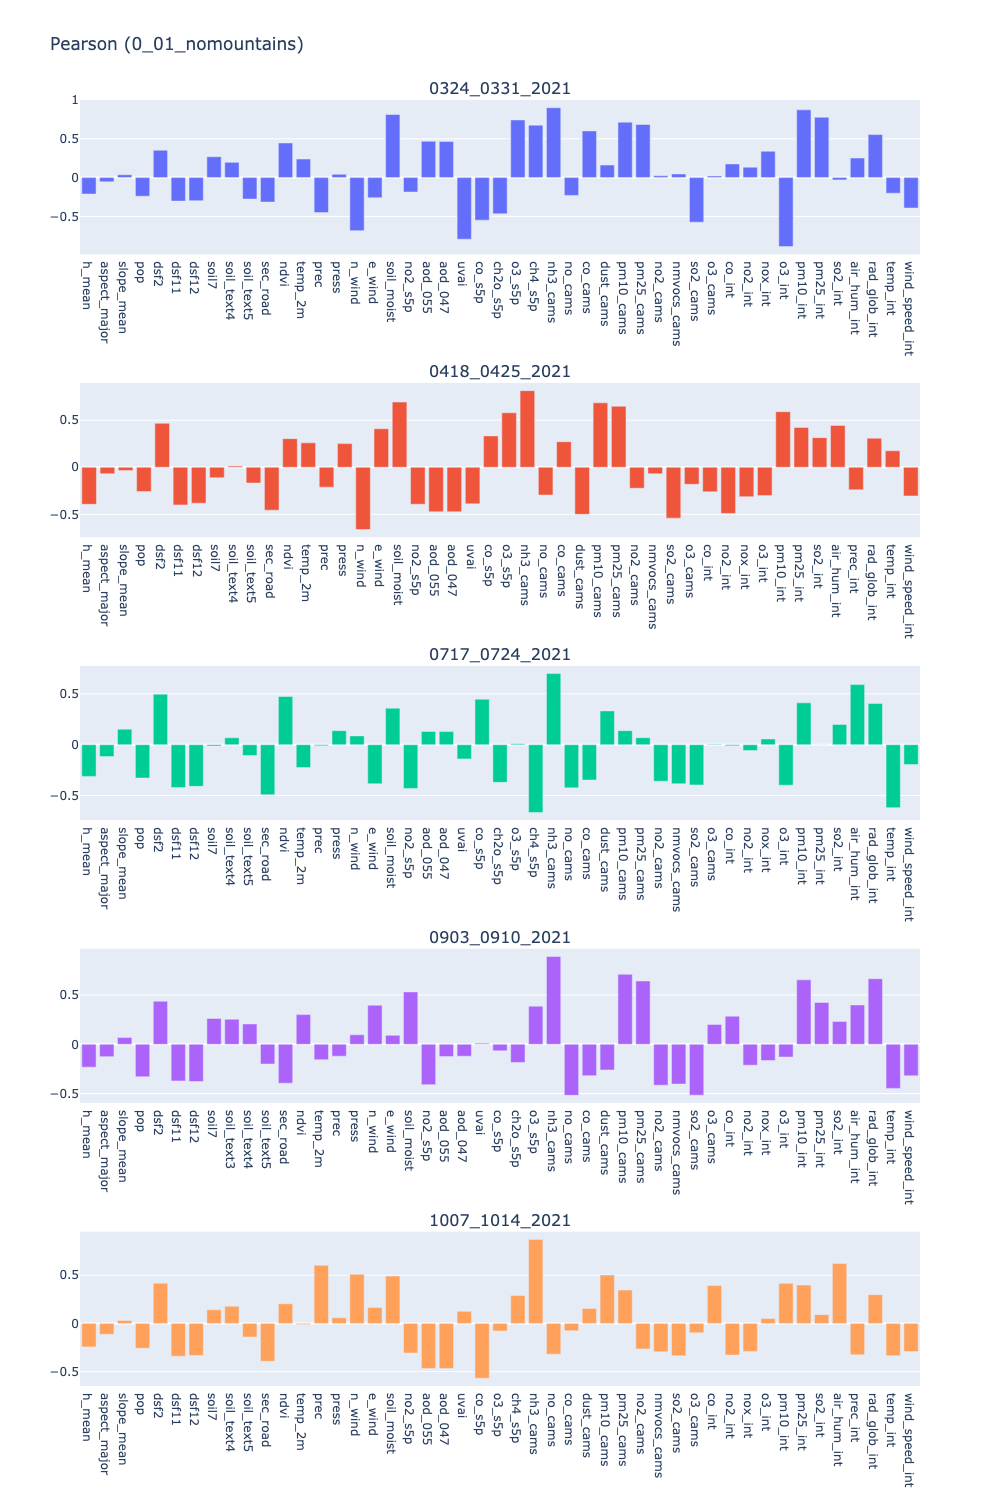
\includegraphics[scale=0.38]{images/tests/0_01_nomountainsnh3_st_pearson.png}
    \caption{Pearson correlation index results with respect to ammonia ('nh3\_st') as target variable, with 1km resolution excluding mountains in each period.}
    
\end{figure}

\section{ML models results}
\subsection{Random Forest}
\begin{table}[H]
\begin{tabular}{lrrrrr}
\toprule
 &  24/03-31/03 &  18/04-25/04 &  17/07-24/07 &  3/09-10/09 &  7/10-14/10 \\
\midrule
 MAE\_sensor &        1.239 &        0.900 &        0.566 &       0.987 &       0.751 \\
RMSE\_sensor &        1.768 &        1.133 &        0.745 &       1.330 &       1.013 \\
 MSE\_sensor &        3.215 &        1.295 &        0.571 &       1.802 &       1.067 \\
  R2\_sensor &        0.883 &        0.812 &        0.722 &       0.834 &       0.858 \\
   MAE\_cams &        7.800 &        6.556 &        2.110 &       3.060 &       3.478 \\
  RMSE\_cams &        9.262 &        7.571 &        2.745 &       3.623 &       4.059 \\
   MSE\_cams &       86.279 &       57.593 &        7.548 &      13.266 &      16.591 \\
    R2\_cams &       -2.147 &       -7.492 &       -2.846 &      -0.258 &      -1.096 \\
\bottomrule
\end{tabular}
\caption{Random Forest prediction for PM2.5 with 10 km resolution, including zones with mountains.}
\end{table}
\begin{table}[H]
\begin{tabular}{lrrrrr}
\toprule
 &  24/03-31/03 &  18/04-25/04 &  17/07-24/07 &  3/09-10/09 &  7/10-14/10 \\
\midrule
 MAE\_sensor &        1.448 &        1.093 &        0.646 &       0.898 &       0.841 \\
RMSE\_sensor &        1.940 &        1.362 &        0.868 &       1.165 &       1.080 \\
 MSE\_sensor &        3.772 &        1.874 &        0.776 &       1.376 &       1.197 \\
  R2\_sensor &        0.872 &        0.766 &        0.683 &       0.870 &       0.793 \\
   MAE\_cams &        8.230 &        7.914 &        1.386 &       3.581 &       3.744 \\
  RMSE\_cams &        9.663 &        8.714 &        1.672 &       4.105 &       4.336 \\
   MSE\_cams &       95.109 &       76.441 &        2.867 &      16.923 &      18.964 \\
    R2\_cams &       -2.312 &       -8.546 &       -0.185 &      -0.632 &      -2.373 \\
\bottomrule
\bottomrule
\end{tabular}
\caption{Random Forest prediction for PM2.5 with 10 km resolution, excluding zones with mountains.}
\end{table}
\begin{table}[H]
\begin{tabular}{lrrrrr}
\toprule
 &  24/03-31/03 &  18/04-25/04 &  17/07-24/07 &  3/09-10/09 &  7/10-14/10 \\
\midrule
 MAE\_sensor &        0.251 &        0.186 &        0.147 &       0.172 &       0.132 \\
RMSE\_sensor &        0.503 &        0.361 &        0.255 &       0.285 &       0.240 \\
 MSE\_sensor &        0.283 &        0.138 &        0.066 &       0.084 &       0.059 \\
  R2\_sensor &        0.992 &        0.985 &        0.981 &       0.994 &       0.993 \\
   MAE\_cams &        8.966 &        7.566 &        1.936 &       3.574 &       3.974 \\
  RMSE\_cams &       10.310 &        8.472 &        2.487 &       4.099 &       4.580 \\
   MSE\_cams &      106.414 &       71.818 &        6.213 &      16.810 &      20.988 \\
    R2\_cams &       -1.821 &       -7.099 &       -0.727 &      -0.180 &      -1.578 \\
\bottomrule
\end{tabular}
\caption{Random Forest prediction for PM2.5 with 1 km resolution, including zones with mountains.}
\end{table}
\begin{table}[H]
\begin{tabular}{lrrrrr}
\toprule
 &  24/03-31/03 &  18/04-25/04 &  17/07-24/07 &  3/09-10/09 &  7/10-14/10 \\
\midrule
 MAE\_sensor &        0.347 &        0.234 &        0.156 &       0.199 &       0.146 \\
RMSE\_sensor &        0.624 &        0.392 &        0.261 &       0.327 &       0.232 \\
 MSE\_sensor &        0.411 &        0.158 &        0.069 &       0.113 &       0.054 \\
  R2\_sensor &        0.990 &        0.985 &        0.982 &       0.993 &       0.991 \\
   MAE\_cams &        9.153 &        8.580 &        1.617 &       3.830 &       4.192 \\
  RMSE\_cams &       10.564 &        9.294 &        1.940 &       4.382 &       4.760 \\
   MSE\_cams &      111.721 &       86.530 &        3.766 &      19.284 &      22.676 \\
    R2\_cams &       -1.682 &       -7.131 &        0.004 &      -0.187 &      -2.674 \\
\bottomrule
\end{tabular}
\caption{Random Forest prediction for PM2.5 with 1 km resolution, excluding zones with mountains.}
\end{table}
\begin{table}[H]
\begin{tabular}{lrrrrr}
\toprule
  &  24/03-31/03 &  18/04-25/04 &  17/07-24/07 &  3/09-10/09 &  7/10-14/10 \\
\midrule
 MAE\_sensor &        4.601 &        2.037 &        2.401 &       3.634 &       1.932 \\
RMSE\_sensor &        5.827 &        2.809 &        3.325 &       5.074 &       2.883 \\
 MSE\_sensor &       35.506 &        8.008 &       11.853 &      26.633 &       9.053 \\
  R2\_sensor &        0.853 &        0.815 &        0.922 &       0.854 &       0.801 \\
   MAE\_cams &       14.956 &       10.748 &        8.166 &      10.326 &       9.163 \\
  RMSE\_cams &       16.458 &       11.633 &       12.027 &      13.395 &      10.105 \\
   MSE\_cams &      272.549 &      135.617 &      149.976 &     194.430 &     102.945 \\
    R2\_cams &       -0.462 &       -2.048 &        0.013 &       0.139 &      -1.066 \\
\bottomrule
\end{tabular}
\caption{Random Forest prediction for NH3 with 10 km resolution, including zones with mountains.}
\end{table}
\begin{table}[H]
\begin{tabular}{lrrrrr}
\toprule
 &  24/03-31/03 &  18/04-25/04 &  17/07-24/07 &  3/09-10/09 &  7/10-14/10 \\
\midrule
 MAE\_sensor &        4.039 &        1.891 &        3.524 &       3.780 &       1.812 \\
RMSE\_sensor &        5.365 &        2.496 &        4.398 &       5.358 &       2.601 \\
 MSE\_sensor &       29.553 &        6.521 &       22.504 &      30.148 &       7.815 \\
  R2\_sensor &        0.895 &        0.829 &        0.814 &       0.848 &       0.911 \\
   MAE\_cams &       15.383 &       10.758 &        8.942 &      10.304 &       9.497 \\
  RMSE\_cams &       16.887 &       11.705 &       12.639 &      13.799 &      10.497 \\
   MSE\_cams &      288.521 &      138.082 &      178.690 &     211.569 &     110.820 \\
    R2\_cams &       -0.022 &       -2.954 &       -0.236 &       0.062 &      -0.547 \\
\bottomrule
\end{tabular}
\caption{Random Forest prediction for NH3 with 10 km resolution, excluding zones with mountains.}
\end{table}
\begin{table}[H]
\begin{tabular}{lrrrrr}
\toprule
 &  24/03-31/03 &  18/04-25/04 &  17/07-24/07 &  3/09-10/09 &  7/10-14/10 \\
\midrule
 MAE\_sensor &        0.450 &        0.180 &        0.505 &       0.669 &       0.345 \\
RMSE\_sensor &        0.954 &        0.327 &        1.120 &       1.803 &       0.785 \\
 MSE\_sensor &        1.065 &        0.147 &        1.861 &       4.244 &       0.732 \\
  R2\_sensor &        0.998 &        0.998 &        0.994 &       0.990 &       0.995 \\
   MAE\_cams &       17.694 &       10.536 &       11.049 &      13.329 &      11.480 \\
  RMSE\_cams &       18.513 &       12.046 &       16.887 &      19.503 &      12.945 \\
   MSE\_cams &      343.112 &      145.433 &      287.761 &     382.879 &     169.030 \\
    R2\_cams &        0.227 &       -1.134 &       -0.044 &       0.124 &      -0.030 \\
\bottomrule
\end{tabular}
\caption{Random Forest prediction for NH3 with 1 km resolution, including zones with mountains.}
\end{table}
\begin{table}[H]
\begin{tabular}{lrrrrr}
\toprule
 &  24/03-31/03 &  18/04-25/04 &  17/07-24/07 &  3/09-10/09 &  7/10-14/10 \\
\midrule
 MAE\_sensor &        0.483 &        0.280 &        0.526 &       0.939 &       0.386 \\
RMSE\_sensor &        0.993 &        0.558 &        1.184 &       2.316 &       0.860 \\
 MSE\_sensor &        1.199 &        0.430 &        1.556 &       6.147 &       1.121 \\
  R2\_sensor &        0.997 &        0.992 &        0.994 &       0.987 &       0.990 \\
   MAE\_cams &       18.401 &       10.414 &       11.746 &      14.180 &      12.012 \\
  RMSE\_cams &       19.196 &       12.126 &       17.744 &      21.241 &      13.697 \\
   MSE\_cams &      368.858 &      147.652 &      323.418 &     456.145 &     188.650 \\
    R2\_cams &        0.136 &       -1.511 &       -0.158 &      -0.001 &      -0.060 \\
\bottomrule
\end{tabular}
\caption{Random Forest prediction for NH3 with 1 km resolution, excluding zones with mountains.}
\end{table}
\subsection{Neural Network by Keras}
\begin{table}[H]
\begin{tabular}{lrrrrr}
\toprule
 &  24/03-31/03 &  18/04-25/04 &  17/07-24/07 &  3/09-10/09 &  7/10-14/10 \\
\midrule
 MAE\_sensor &        2.127 &        1.581 &        0.847 &       1.516 &       1.268 \\
RMSE\_sensor &        2.643 &        2.008 &        1.046 &       1.912 &       1.591 \\
 MSE\_sensor &        7.097 &        4.064 &        1.108 &       3.743 &       2.578 \\
  R2\_sensor &        0.750 &        0.358 &        0.408 &       0.649 &       0.672 \\
   MAE\_cams &        7.800 &        6.554 &        2.113 &       3.060 &       3.478 \\
  RMSE\_cams &        9.262 &        7.571 &        2.720 &       3.598 &       4.067 \\
   MSE\_cams &       86.279 &       57.562 &        7.565 &      13.266 &      16.591 \\
    R2\_cams &       -2.147 &       -8.102 &       -3.386 &      -0.239 &      -1.158 \\
\bottomrule
\end{tabular}
\caption{Neural Network prediction for PM2.5 with 10 km resolution, including zones with mountains.}
\end{table}
\begin{table}[H]
\begin{tabular}{lrrrrr}
\toprule
 &  24/03-31/03 &  18/04-25/04 &  17/07-24/07 &  3/09-10/09 &  7/10-14/10 \\
\midrule
 MAE\_sensor &        1.864 &        1.605 &        0.871 &       1.308 &       1.052 \\
RMSE\_sensor &        2.257 &        1.955 &        1.100 &       1.612 &       1.327 \\
 MSE\_sensor &        5.188 &        3.894 &        1.279 &       2.696 &       1.890 \\
  R2\_sensor &        0.826 &        0.538 &        0.457 &       0.731 &       0.653 \\
   MAE\_cams &        8.243 &        7.907 &        1.383 &       3.581 &       3.744 \\
  RMSE\_cams &        9.717 &        8.713 &        1.677 &       4.086 &       4.342 \\
   MSE\_cams &       95.313 &       76.364 &        2.859 &      16.923 &      18.964 \\
    R2\_cams &       -2.281 &       -8.213 &       -0.193 &      -0.561 &      -2.351 \\
\bottomrule
\end{tabular}
\caption{Neural Network prediction for PM2.5 with 10 km resolution, excluding zones with mountains.}
\end{table}
\begin{table}[H]
\begin{tabular}{lrrrrr}
\toprule
 &  24/03-31/03 &  18/04-25/04 &  17/07-24/07 &  3/09-10/09 &  7/10-14/10 \\
\midrule
 MAE\_sensor &        1.546 &        0.970 &        0.721 &       1.170 &       1.040 \\
RMSE\_sensor &        1.997 &        1.340 &        0.988 &       1.528 &       1.325 \\
 MSE\_sensor &        4.079 &        1.831 &        0.991 &       2.339 &       1.776 \\
  R2\_sensor &        0.891 &        0.798 &        0.727 &       0.839 &       0.779 \\
   MAE\_cams &        8.966 &        7.567 &        1.936 &       3.574 &       3.974 \\
  RMSE\_cams &       10.314 &        8.473 &        2.490 &       4.096 &       4.579 \\
   MSE\_cams &      106.423 &       71.820 &        6.214 &      16.811 &      20.987 \\
    R2\_cams &       -1.840 &       -6.979 &       -0.735 &      -0.157 &      -1.585 \\
\bottomrule
\end{tabular}
\caption{Neural Network prediction for PM2.5 with 1 km resolution, including zones with mountains.}
\end{table}
\begin{table}[H]
\begin{tabular}{lrrrrr}
\toprule
 &  24/03-31/03 &  18/04-25/04 &  17/07-24/07 &  3/09-10/09 &  7/10-14/10 \\
\midrule
 MAE\_sensor &        1.508 &        0.875 &        0.739 &       0.793 &       0.593 \\
RMSE\_sensor &        1.995 &        1.174 &        0.972 &       1.002 &       0.836 \\
 MSE\_sensor &        4.033 &        1.396 &        0.967 &       1.050 &       0.704 \\
  R2\_sensor &        0.904 &        0.868 &        0.737 &       0.937 &       0.888 \\
   MAE\_cams &        9.153 &        8.581 &        1.617 &       3.830 &       4.192 \\
  RMSE\_cams &       10.565 &        9.298 &        1.939 &       4.386 &       4.761 \\
   MSE\_cams &      111.720 &       86.539 &        3.766 &      19.282 &      22.673 \\
    R2\_cams &       -1.627 &       -7.082 &       -0.006 &      -0.181 &      -2.616 \\
\bottomrule
\end{tabular}
\caption{Neural Network prediction for PM2.5 with 1 km resolution, excluding zones with mountains.}
\end{table}
\begin{table}[H]
\begin{tabular}{lrrrrr}
\toprule
 &  24/03-31/03 &  18/04-25/04 &  17/07-24/07 &  3/09-10/09 &  7/10-14/10 \\
\midrule
 MAE\_sensor &        5.441 &        2.433 &        4.971 &       5.729 &       3.219 \\
RMSE\_sensor &        6.896 &        3.283 &        7.496 &       7.618 &       4.613 \\
 MSE\_sensor &       49.263 &       11.191 &       60.601 &      70.032 &      21.714 \\
  R2\_sensor &        0.785 &        0.722 &        0.618 &       0.726 &       0.722 \\
   MAE\_cams &        6.660 &        4.050 &        7.537 &       6.583 &       2.601 \\
  RMSE\_cams &        8.289 &        5.473 &       10.610 &       9.773 &       3.662 \\
   MSE\_cams &       69.718 &       31.198 &      115.937 &     102.716 &      13.809 \\
    R2\_cams &        0.680 &        0.217 &        0.212 &       0.546 &       0.822 \\
\bottomrule
\end{tabular}
\caption{Neural Network prediction for NH3 with 10 km resolution, including zones with mountains.}
\end{table}
\begin{table}[H]
\begin{tabular}{lrrrrr}
\toprule
 &  24/03-31/03 &  18/04-25/04 &  17/07-24/07 &  3/09-10/09 &  7/10-14/10 \\
\midrule
 MAE\_sensor &        4.625 &        2.297 &        4.749 &       5.573 &       3.139 \\
RMSE\_sensor &        5.405 &        2.988 &        5.801 &       7.571 &       4.557 \\
 MSE\_sensor &       33.849 &        9.630 &       37.672 &      58.766 &      25.848 \\
  R2\_sensor &        0.867 &        0.710 &        0.702 &       0.704 &       0.675 \\
   MAE\_cams &        7.283 &        4.559 &        8.412 &       7.581 &       3.033 \\
  RMSE\_cams &        8.867 &        6.016 &       11.236 &      10.874 &       4.072 \\
   MSE\_cams &       78.979 &       36.499 &      135.704 &     123.934 &      16.818 \\
    R2\_cams &        0.710 &       -0.106 &       -0.034 &       0.425 &       0.591 \\
\bottomrule
\end{tabular}
\caption{Neural Network prediction for NH3 with 10 km resolution, excluding zones with mountains.}
\end{table}
\begin{table}[H]
\begin{tabular}{lrrrrr}
\toprule
 &  24/03-31/03 &  18/04-25/04 &  17/07-24/07 &  3/09-10/09 &  7/10-14/10 \\
\midrule
 MAE\_sensor &        3.064 &        1.920 &        4.194 &       2.612 &       2.140 \\
RMSE\_sensor &        3.953 &        3.010 &        5.592 &       3.497 &       2.518 \\
 MSE\_sensor &       17.004 &        9.733 &       31.882 &      12.736 &       8.747 \\
  R2\_sensor &        0.962 &        0.861 &        0.879 &       0.968 &       0.953 \\
   MAE\_cams &        8.197 &        4.031 &       10.073 &       9.247 &       4.327 \\
  RMSE\_cams &       10.860 &        6.169 &       14.998 &      15.436 &       7.145 \\
   MSE\_cams &      118.847 &       38.357 &      225.879 &     243.268 &      51.953 \\
    R2\_cams &        0.736 &        0.456 &        0.180 &       0.445 &       0.695 \\
\bottomrule
\end{tabular}
\caption{Neural Network prediction for NH3 with 1 km resolution, including zones with mountains.}
\end{table}


\begin{table}[H]
\begin{tabular}{lrrrrr}
\toprule
 &  24/03-31/03 &  18/04-25/04 &  17/07-24/07 &  3/09-10/09 &  7/10-14/10 \\
\midrule
 MAE\_sensor &        1.904 &        2.287 &        3.126 &       2.743 &       3.146 \\
RMSE\_sensor &        2.570 &        3.341 &        4.205 &       3.841 &       4.465 \\
 MSE\_sensor &        6.867 &       11.579 &       18.068 &      16.405 &      21.579 \\
  R2\_sensor &        0.984 &        0.800 &        0.927 &       0.965 &       0.852 \\
   MAE\_cams &        9.253 &        4.560 &       11.334 &      11.259 &       5.461 \\
  RMSE\_cams &       11.641 &        6.600 &       15.831 &      17.476 &       8.145 \\
   MSE\_cams &      135.675 &       43.816 &      257.910 &     306.085 &      67.695 \\
    R2\_cams &        0.692 &        0.254 &        0.058 &       0.342 &       0.631 \\
\bottomrule
\end{tabular}
\caption{Neural Network prediction for NH3 with 1 km resolution, excluding zones with mountains.}
\end{table}










